\chapter{Introduction}

\KOMAoptions{headsepline=true}
\lohead{\leftmark}
\rehead{\rightmark}
\pagenumbering{arabic}
\setcounter{page}{1}

\begin{chapterinfo}
    This chapter is a general introduction to accelerator physics.
    The goal of this introduction is to collect all the necessary tools that are needed to develop
    the methods and algorithms presented in the main part of this thesis.
    Therefore we need a sound understanding of linear beam optics, 
    $\beta$~function, phase, coupling and chromaticity.
    Only a brief summary of the vast field of accelerator physics can be given in the scope of this
    thesis. The interested reader may consult some of the great introductory works of the field, e.g.
    \cite{WolskiBook}.

    Also the normal form approach shall be introduced here as it is needed to calculate optics
    parameters from Hamiltonian terms in chapter~\ref{ch_localobs}.

\end{chapterinfo}

\section{A word on notation}

Accelerator physics is a field, for sure not the only one, with notoriously bad notation and conventions.
In multiple cases the same symbol is used to describe two or more completely different quantities.
Keeping the notation of a work like this PhD thesis consistent is not an easy task on its own. Less so
in the given situation.
Therefore this little prolog serves in guiding the reader through the notations and conventions adopted
throughout this thesis.

\textbf{Planes} We describe the motion of the particles and beams in the regime of \emph{transverse beam dynamics} with
two transverse planes $x$ and $y$.
So we have to distinguish optical functions and variables by plane: $x, y, \beta_x, \alpha_x, \phi_x$.

Most of the time however it is of no importance in which plane the equations
are expressed or we work for an extended period in the same plane.
In those cases, the index denoting the plane will be dropped. 

\textbf{Vectors} are denoted by an italic letter with an arrow above. Phase space \textbf{coordinates} are
usually denoted by lowercase latin letters ($\vec{x}, \vec{v}, \vec{p}$) with the exception of normal form coordinates
which are greek lowarcase letters ($\vec{\zeta}, \vec{\xi}$). \textbf{Fields} are denoted by capital
latin letters ($\vec{E}, \vec{B}$).

\textbf{Matrices} are denoted by bold face letters, usually capital latin $\mat{M}, \mat{V}$.

\section{Beam Optics}

Charged particle beams in an accelerator can be bent, focused, defocused and can be subject to effects
like dispersion and chromaticity very much like light beams. Therefore the term \emph{optics} is
generally used to describe the movement and behaviour of particle beams around the accelerator.

Important optics parameters are described in this section like $\beta$~function, betatron phase and
transverse coupling.
The discription is limited to single particle dynamics. Effects of the particles on each other are
neglected for the sake of the studies in this thesis.

\subsection{Linear Beam Dynamics}

Linear beam dynamics studies the effect of linear electromagnetic fields on the particles.
Thus, primarily only drift spaces, bending magnets and (de)focusing magnets are considered.
In this case only Lorentz force acts on the particles\footnote{Of course also other forces like gravity
act on the particle. But those are negligible.}:

\begin{equation}
    \vec{F} = q\left(\vec{E} + \vec{v} \times \vec{B}\right)
    \fstop
    \label{eq_lorentz_force}
\end{equation}

A dipole with a constant magnetic field $B_y$ bends the particles trajectory into an arc of radius $\rho$

\begin{equation}
    \rho = \frac{p}{qB_y}
    \fstop
    \label{eq_acc_radius}
\end{equation}

It is useful to describe the motion in a circular accelerator in a co-moving reference frame as
depictet in \figref{fig_frenet_serret} where the cartesian coordinates $\{x', y', z'\}$ are
transformed into a system $\{x,y,s\}$ with the properties:

\begin{align}
    \hat{s} &\parallel \text{design orbit}\notag\\
    \hat{y} &= \hat{y}'\notag\\
    \hat{x} &= \hat{y} \times \hat{s}
\end{align}


\begin{figure}[h]
    \includestandalone{frenetserret}
    \caption{
        The Frenet-Serret coordinate system which is moving along the design orbit of particles
        in the accelerator.
    }
    \label{fig_frenet_serret}
\end{figure}

In this coordinate system the motion of a particle in a circular accelerator is described by Hill's
differential equation:

\begin{equation}
    \frac{\der^2 q}{\der s^2} + k(s)q = 0
    %\fstop
    \label{eq_hills}
\end{equation}

where $q \in \{x,y\}$ is the transverse coordinate and $k(s)$ is the linear magnet strength at
position $s$.

A solution that satisfies \eqref{eq_hills} is

\begin{equation}
    q(s) = A_q(s) \cos\left(\phi_q(s) + \phi_{q,0} \right)
    \label{eq_betatron_osc}
\end{equation}
where the $s$-dependent amplitude of the oscillation can be split:
\begin{equation}
    A_q(s) = \sqrt{2I_q \beta_q(s)}
    \fstop
    \label{eq_betatron_ampl}
\end{equation}
$\beta_q(s)$ is the $s$-dependent part of the amplitude, called $\beta$~function. $\beta(s)$ and 
$\phi(s)$ are periodic with the circumference of the ring $C$.

$\phi(s)$ is called the \emph{betatron phase} and satisfies the following property:

\begin{equation}
    \phi(s_1) - \phi(s_0) = \int\limits_{s_0}^{s_1} \frac{1}{\beta(s)}\der s
    \fstop
    \label{eq_phase}
\end{equation}

For convenience later we introduce the following short-hand notation:

\begin{equation}
    \phi_{q,ab} = \phi_q(s_b) - \phi_q(s_a)
\end{equation}
which is the \emph{phase advance} between position $s_a$ and $s_b$.

Solutions of \eqref{eq_hills} for linear lattice elements can be expressed in matrix form

\begin{equation}
    \begin{pmatrix}
        q_1\\
        q_1'
    \end{pmatrix}
    =
    \begin{pmatrix}
        m_{11} & m_{12} \\
        m_{21} & m_{22}
    \end{pmatrix}
    \begin{pmatrix}
        q_0\\
        q_0'
    \end{pmatrix}
    \fstop
    \label{eq_matrix_element}
\end{equation}
The matrix 
\begin{equation}
    \mat{M} = 
    \begin{pmatrix}
        m_{11} & m_{12} \\
        m_{21} & m_{22}
    \end{pmatrix}
    \label{eq_trmat}
\end{equation}
is called the \emph{transfer matrix}. It describes the transformation
of phase space when going from one position $s_0$ in the lattice to another $s_1$.

A general form of \eqref{eq_trmat} is 

\begin{equation}
    \begin{pmatrix}
        \sqrt{\frac{\beta_b}{\beta_a}}(\cos\phi_{ab} + \alpha_a \sin\phi_{ab}) &
        \sqrt{\beta_a\beta_b} \sin\phi_{ab} \\
        \frac{\alpha_a - \alpha_b}{\sqrt{\beta_a\beta_b}}\cos\phi_{ab} - \frac{b+\alpha_a\alpha_b}{\sqrt{\beta_a\beta_b}}\sin\phi_{ab} &
        \sqrt{\frac{\beta_a}{\beta_b}}(\cos\phi_{ab} - \alpha_b\sin\phi_{ab})
    \end{pmatrix}
    \label{eq_trmat_01}
\end{equation}
where the quantity

\begin{equation}
    \alpha(s) = -\frac{\der \beta(s)}{2 \der s}
    \label{eq_alpha}
\end{equation}

is called $\alpha$~\emph{function}.

A special example of the transfermatrix is the one between a position $s_i$ and the position but in
the following turn, called \emph{one-turn map}, which can be retrieved by setting $\beta_a = \beta_b $
and $\alpha_a = \alpha_b$ in \eqref{eq_trmat_01}:

\begin{equation}
    M_i = \begin{pmatrix}
        \cos(2\pi Q_q) + \alpha_a \sin(2\pi Q_q) & \beta_a\sin(2\pi Q_q) \\
        -\frac{1+\alpha_a^2}{\beta_a}\sin(2\pi Q_q) & \cos(2\pi Q_q) - \alpha_a\sin(2\pi Q_q)
    \end{pmatrix}
    \fstop
\end{equation}
The value $Q_q$ is an important lattice paramter called the \emph{betatron tune}.



\section{Resonance driving terms}

In order to derive optics parameters from Hamiltonian terms the normal form approach -- classically
used to describe non-linear optics -- is useful. 

The transfer map of a general (non-linear) element is given by
\begin{equation}
    M= \e{:H_w(s):}R
\end{equation}
where $R$ is the simple rotation of linear components and the Hamiltonian term $H_w(s)$ is given by
\begin{equation}
    H_w(s) = \sum\limits_n\sum\limits_{jklm} h_{w,jklm}\expi{(j-k)\phi_{w,x}}
\end{equation}

\begin{equation}
    f_{jklm}=\sum\limits_{n}\sum\limits_{j+k+l+m=n} \frac{h_{jklm} }{1-\e{2\pi i [(j-k)Q_x+(l-m)Q_y]}}
\end{equation}


\section{Forced motion}

\section{The Large Hadron Collider}

The Large Hadron Collider is the world's largest particle accelerator with the highest center of mass
energy per charge unit. It has a circumference of $\SI{27}{km}$ and is situated at the French-Swiss 
border near Geneva. The top energy for protons is $\SI{7}{TeV}$
and in the lead ion run of 2018 a beam energy of $\SI{6.37}{Z TeV}$ was achieved.

The particles pass through various pre-accelerators where they are accelerated in steps before being
injected in the LHC at $\SI{450}{GeV}$. The complete accelerator complex at CERN is sketched in
\figref{fig_cern_acc_cmplx}.

\begin{figure}[h]
    \centering
    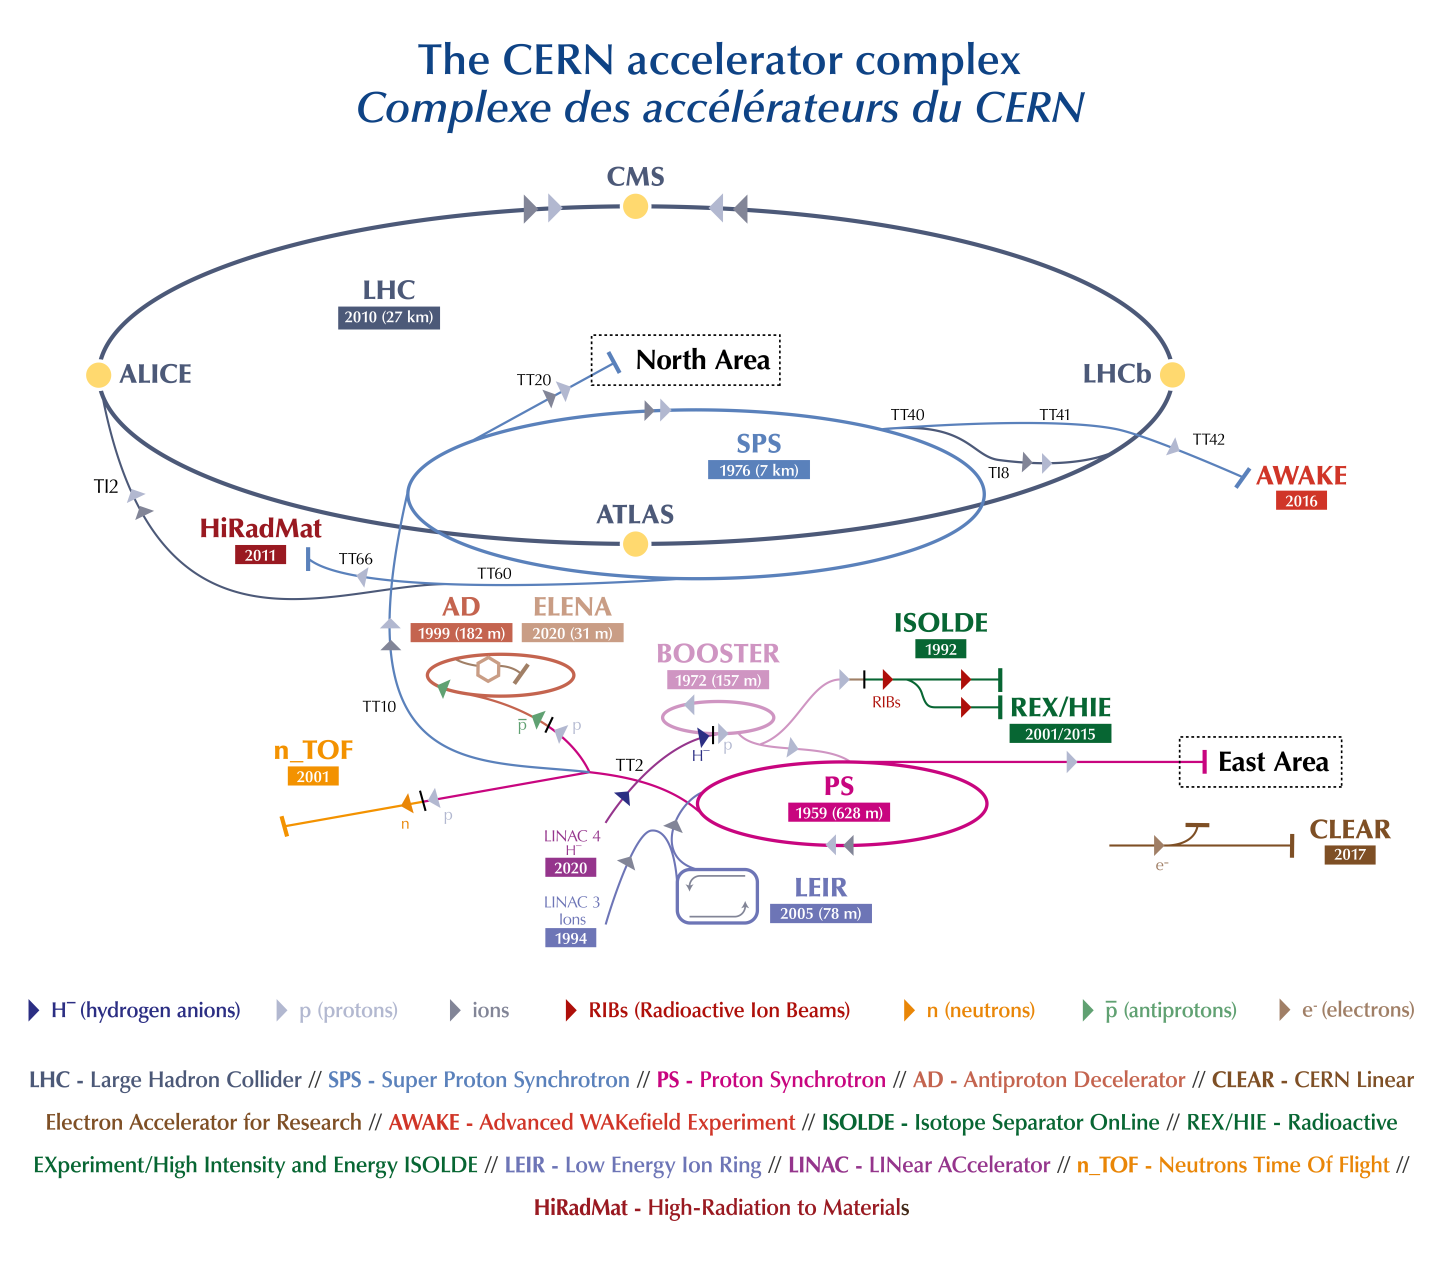
\includegraphics[width=\textwidth]{CCC-v2019-final-white_small}
    \caption{CERN has various accelerators and decelerators. H$^-$ ions are pre-accelerated
    in LINAC2 (LINAC4 in the future) and passed to PSBooster, PS, SPS and finally injected into
    the LHC. Image credit: \cite{CERN_AccCmplx}}
    \label{fig_cern_acc_cmplx}
\end{figure}
